\documentclass[DIV=12, ngerman, fontsize=12pt, parskip=half]{scrreprt}

\usepackage[utf8]{inputenc}
\usepackage[ngerman]{babel}
\usepackage[T1]{fontenc}
\usepackage{lmodern}
\usepackage{microtype}
\usepackage{graphicx}
\usepackage{csquotes}
\usepackage[onehalfspacing]{setspace}
\usepackage[table,xcdraw]{xcolor}
\usepackage{tabularx}
\usepackage{mathtools}
\usepackage{amsmath}
\usepackage{amssymb}
\usepackage{float}
\usepackage{array}
\usepackage{subcaption}
\usepackage{bbold}
\usepackage{pdfpages}
%\usepackage{subfig}
\clubpenalty10000
\widowpenalty10000

\begin{document}
	
	\setcounter{chapter}{1-1}
	
	\begin{center}
		
		\huge
		\textbf{Machine Learning I - Sheet 3} 
	\end{center}
	
	
	\begin{center}
		\Large
		\text{08.02.2020}
	\end{center}
	
	
	\begin{center}
		\large
		\text{Johannes Groß, 2036852, BSc Physik}\\
		\text{Leonard Bleiziffer, 2038588, BSc Physik}	
		
	\end{center}
	
	\thispagestyle{empty}
	%	\tableofcontents 
	\thispagestyle{empty}
	
	\vspace{0cm}
	
	{\let\clearpage\relax \chapter{Self organizing maps}}
	A one dimensional self organizing map is used to solve the traveling salesman problem. In our example, we tried to find the shortest possible route for visiting all the beergardens of Regensburg. The GPS coordinates of the beergardens are used to place them in a two dimensional space. \\
	The code provided in the github repository https://github.com/DiegoVicen/ntnu-som was used to initialize, train and plot the SOM. The code was only changed to be able to train the SOM on the beergarden data. \\
	The used SOM has eight neurons per beergarden, the neighborhood was modeled with a Gaussian and the neighborhood radius as well as the learning rate decayed exponentially. Tuning the decay parameters of the radius and the learning rate has a great impact on both, the final solution and the number of iterations until convergence. Both decays should be chosen as fast as possible to speed up convergence, but when they are too rapid, the final solution will be far from optimal because too many neurons are dead too soon.
	
	\begin{figure}[H]
		\begin{center}
			\begin{minipage}[t]{0.45\textwidth}
				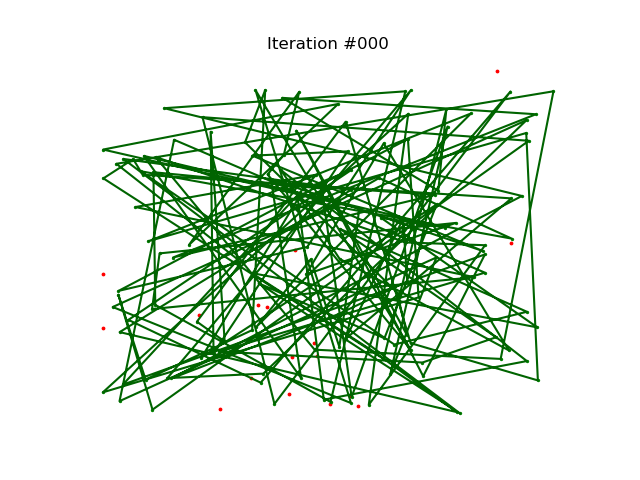
\includegraphics[width=\textwidth]{TSP_0}
			\end{minipage}
			\begin{minipage}[t]{0.45\textwidth}
				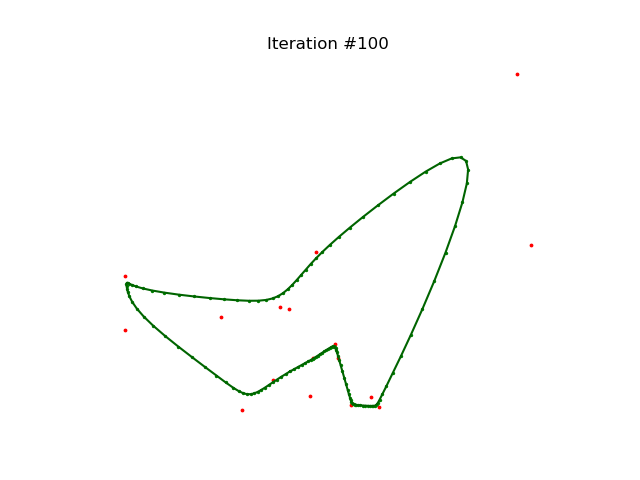
\includegraphics[width=\textwidth]{TSP_100}
			\end{minipage}
			\begin{minipage}[b]{0.45\textwidth}
				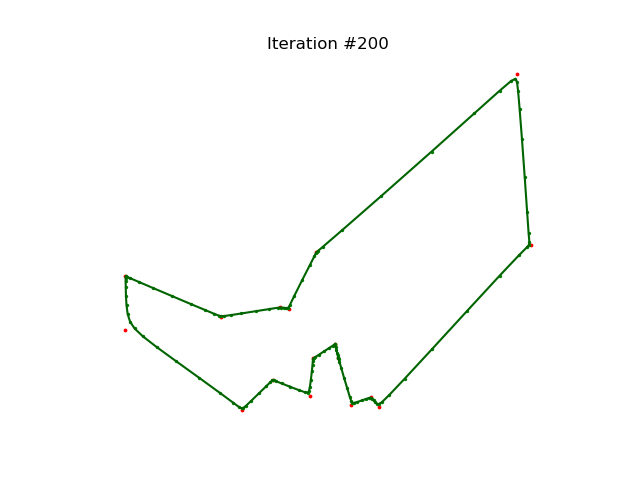
\includegraphics[width=\textwidth]{TSP_200}
			\end{minipage}
			\begin{minipage}[b]{0.45\textwidth}
			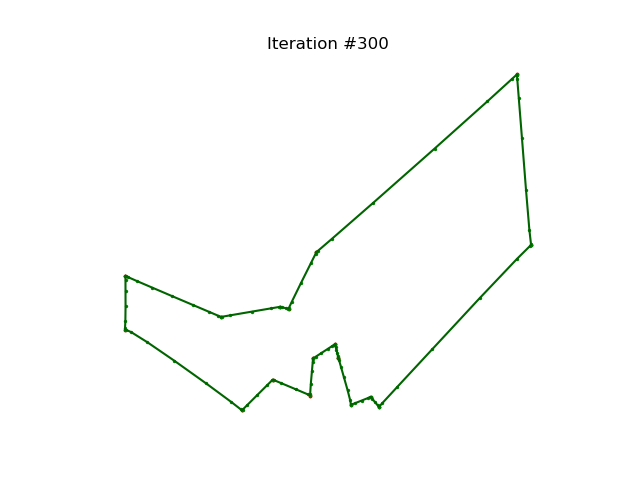
\includegraphics[width=\textwidth]{TSP_300}
			\end{minipage}
			\caption{Snapshots of the solution from random initialization until convergence.}
		\end{center}
	\end{figure}


	\chapter{Multi layer perceptron}
	
	\section{Regression}
	A multi layer perceptron (MLP) was used to approximate a non-linear function $f(x)$. Value pairs of $x$ and $f(x)$ were provided for $x\in [0,20]$. The MLP was trained with $tanh$ and $logistic$ as activation functions and with different numbers of hidden layers and hidden neurons. \\
	In both cases the optimal architecture was 1 hidden layer with 2 neurons in it. This leads to an optimal result with the least complexity. However, in general the two activation functions react differently to different architectures. It can be observed that adding more hidden layers, while increasing the complexity, is not necessarily beneficial to the performance. Furthermore, we noticed that increasing the number of hidden layers demands an increase of neurons per layer in order to achieve good accuracy again. Of course, this further increases the compute time of the MLP. The complexity of the MLP is given by $O(n\cdot h_1\cdot ...\cdot h_k\cdot i)$, where $n$ is the number of samples, $h_j$ is the number of neurons in the $j-th$ hidden layer and $i$ is the number of iterations. \\
	The notation for the architecture $(i,j)$ means that the first hidden layer contains $i$ neurons and the second hidden layer contains $j$ neurons.
	
	\begin{figure}[H]
		\begin{center}
			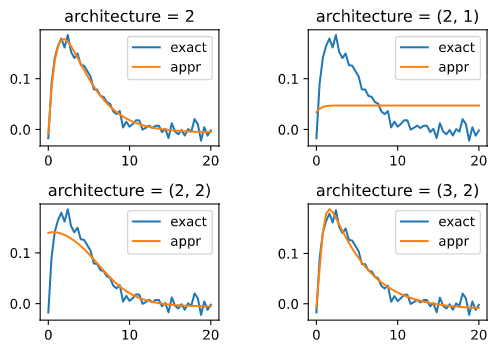
\includegraphics[scale=0.54]{regr_tanh}
			\caption{Plots for the estimation with the activation function $tanh$.}
		\end{center}
	\end{figure}
	\begin{figure}[H]
		\begin{center}
			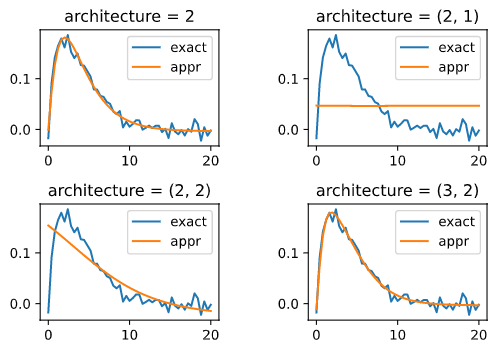
\includegraphics[scale=0.54]{regr_logistic}
			\caption{Plots for the estimation with the activation function $logistic$.}
		\end{center}
	\end{figure}


	\section{Classification}
	In this task, a MLP classifier was trained on the 'EMG Physical Action Data Set' from sheet 2 task 1. The architecture was optimized for the accuracy and compared to the support vector machine (SVM) and random forest (RF). The $logistic-function$ was used as activation as it performed better than $tanh$. The following tables show the performance of the MLP for different architectures, once with and once without standardizing the features by removing the mean and scaling to unit variance. The MLPs with the highest accuracies are colored:
	
	\begin{table}[H]
		\begin{center}
		\begin{tabular}{|l|l|l|}
			\hline
						  & Accuracy & Time {[}s{]} \\ \hline
			(50)          & 0.7806   & 12.93        \\ \hline
			(100)         & 0.7679   & 22.21        \\ \hline
			(200)         & 0.7811   & 38.11        \\ \hline
			(500)         & 0.7976   & 125.96       \\ \hline
			(50,50)       & 0.8327   & 47.86        \\ \hline
			\cellcolor[HTML]{FFC702}
			(100,100)     & 0.8404   & 67.93        \\ \hline
			(200,200)     & 0.8345   & 337.75       \\ \hline
			(50,50,50)    & 0.8203   & 36.69        \\ \hline
			(100,100,100) & 0.8302   & 95.60        \\ \hline
			(200,200,200) & 0.8218   & 395.98       \\ \hline
		\end{tabular}
		\caption{Results for different architectures on the non-standardized data set.}
		\end{center}
	\end{table}

	\begin{table}[H]
	\begin{center}
		\begin{tabular}{|l|l|l|}
			\hline
						  & Accuracy & Time {[}s{]} \\ \hline
			(50)          & 0.8242   & 59.20        \\ \hline
			(100)         & 0.8423   & 132.14        \\ \hline
			(200)         & 0.8391   & 194.94        \\ \hline
			(500)         & 0.8476   & 375.64       \\ \hline
			\cellcolor[HTML]{34FF34}
			(50,50)       & 0.8547   & 172.25        \\ \hline 
			(100,100)     & 0.8512   & 266.16        \\ \hline
			(200,200)     & 0.8478   & 524.11       \\ \hline
			(50,50,50)    & 0.8505   & 217.53        \\ \hline
			(100,100,100) & 0.8375   & 382.80        \\ \hline
			(200,200,200) & 0.8413   & 626.55       \\ \hline
		\end{tabular}
		\caption{Results for different architectures on the standardized data set.}
	\end{center}
	\end{table}
	
	Interestingly, the MLP classifier achieved a better accuracy on the standardized data, but only at the cost of a lot more compute time.\\
	The following table compares the three different algorithms. RF achieves the highest accuracy and takes the least amount of time. Therefore, RF comes out as a clear winner on this data set. Between SVM and MLP one has to trade off between accuracy and computing time. The table shows the values for the green colored MLP, the one with the highest accuracy.
	
	\begin{table}[H]
		\begin{center}
			\begin{tabular}{|l|l|l|}
				\hline
							  & Accuracy & Time {[}s{]} \\ \hline
				SVM  		  & 0.7892   & 28.50        \\ \hline
				RF  	 	  & 0.8774   & 6.52         \\ \hline
				MLP 		  & 0.8547   & 172.25        \\ \hline
			\end{tabular}
		\end{center}
	\end{table}
	

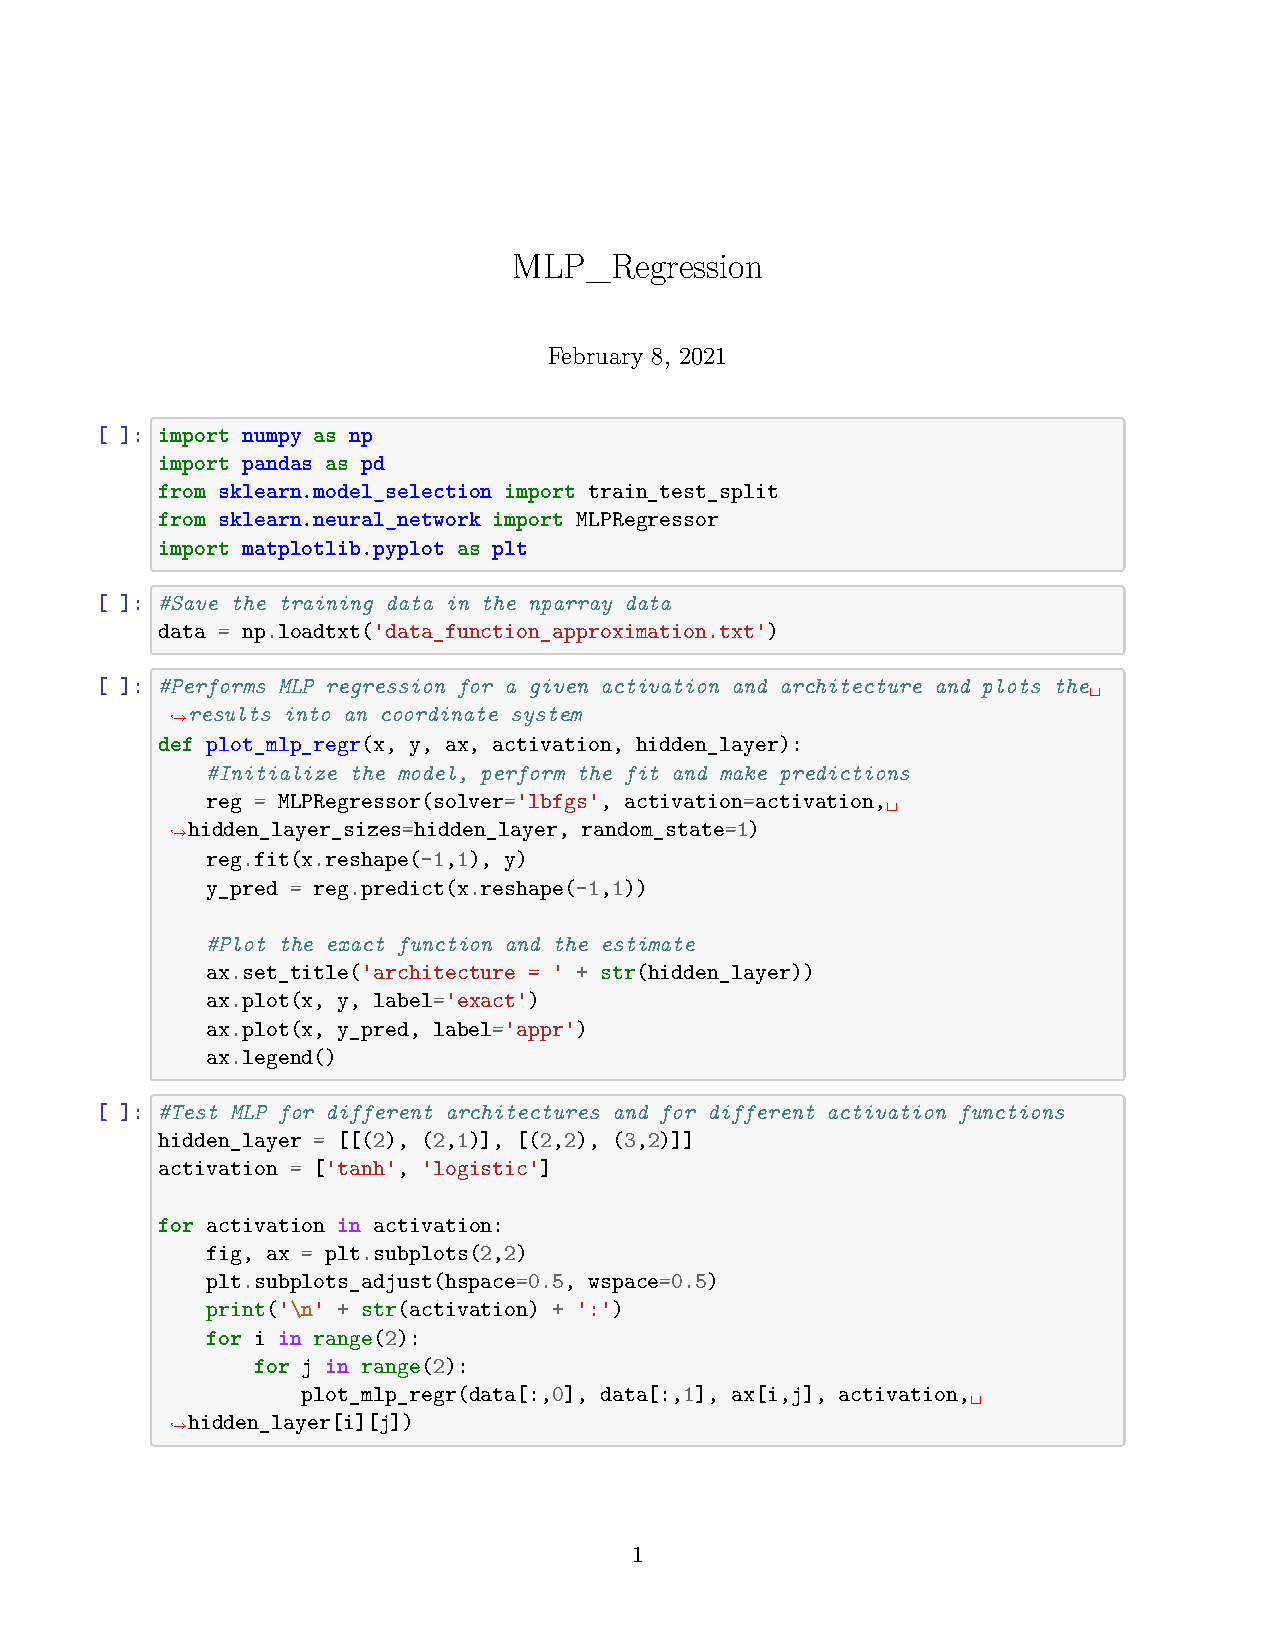
\includepdf[pages=-]{MLP_Regression}
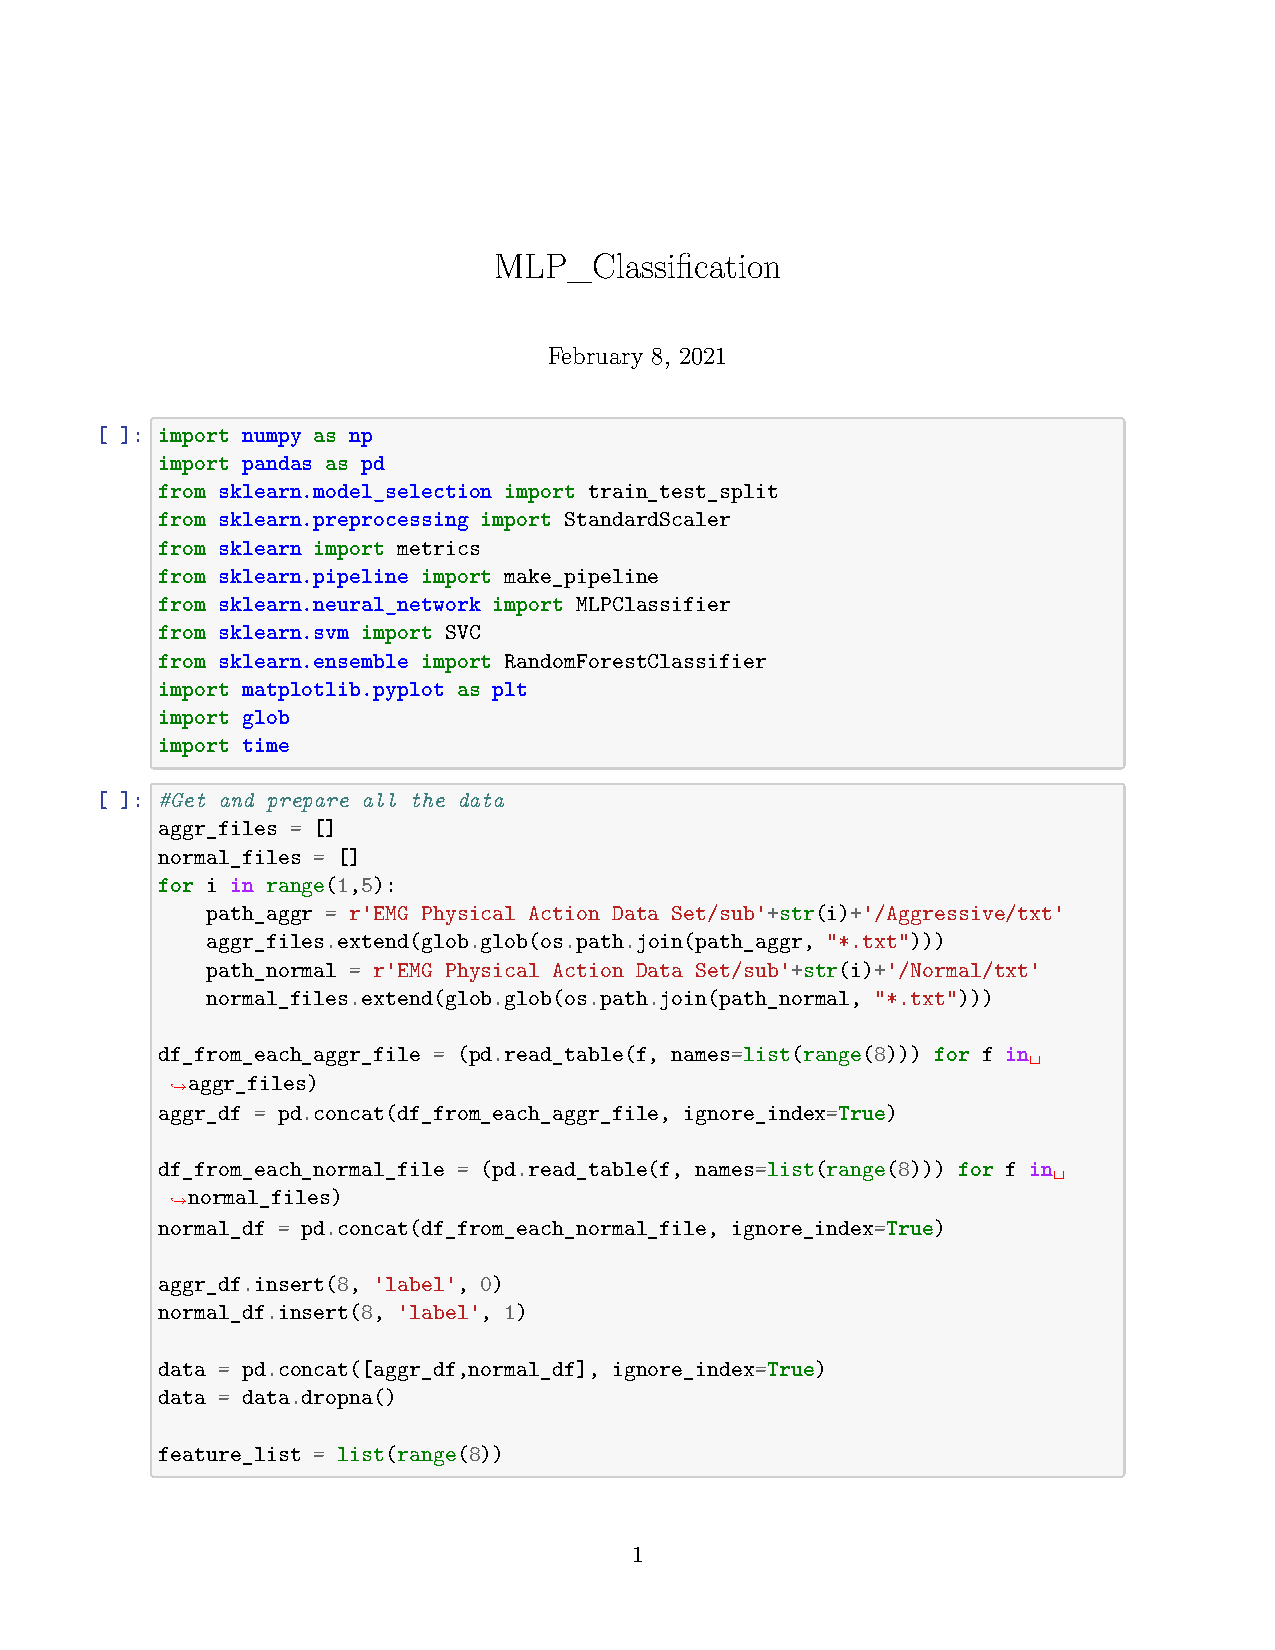
\includepdf[pages=-]{MLP_Classification}

	
\end{document}